\chapter{Implementasi dan Pengujian}
\label{chap:implementasiPengujian}

Bab ini terdiri atas implementasi, pengujian, dan masalah yang dihadapi.

\section{Implementasi}
\subsection{Lingkungan Implementasi}
Berikut adalah spesifikasi  {\it laptop} yang digunakan untuk implementasi:
\begin{enumerate}
	\item {\it Processor} : Intel (R) Core (TM) i7-2630QM
	\item {\it Memory} : 8192 MB RAM
	\item {\it Operating System} : Windows 10 Home 64-bit
\end{enumerate}

Berikut adalah spesifikasi perangkat lunak yang digunakan untuk implementasi:
\begin{enumerate}
	\item IDE : version 4.12.0
	\item Bahasa Pemrograman : Java
	\item Java Library : Java 1.8.0\_ 191
\end{enumerate}

Berikut adalah spesifikasi node sensor yang digunakan untuk implementasi:
\begin{enumerate}
    \item Nama : Preon32
    \item \textit{Processor} : Cortex-M3
    \item \textit{Operating System} : PreonVM
    \item Penyimpanan Sistem : 64 kByte SRAM
    \item Penyimpanan Data : 256 kByte Flash
    \item Pita frekuensi : 2400.0 - 2483.5 MHz
    \item Jangkauan : 250 meter (luar ruangan) dan 30 meter (dalam ruangan)
    \item Sensor-sensor : Sensor suhu, sensor cahaya, sensor kelembaban, sensor tekanan udara, dan sensor getaran.
\end{enumerate}

\subsection{Hasil Implementasi Kelas}
Berdasarkan pembahasan pada bab \ref{chap:perancangan}, terdapat kelas - kelas yang diimplementasi di sensor node yaitu kelas {\it Accelerometer}, kelas {\it Complex}, kelas {\it FFT}, kelas {\it SenseController}, kelas {\it ShortTimeFourierTransform}, kelas {\it SNManager} dan kelas {\it BSManager}. Kelas - kelas yang diimplementasi di sensor node akan diatur oleh kelas {\it SNManager} atau {\it BSManager} jika sensor node tersebut adalah {\it base station}. Selain dari kelas - kelas tersebut, terdapat kelas yang diimplementasi di komputer sebagai penghubung antara 
{\it base station} dengan komputer.

\subsubsection{Kelas Accelerometer}
Pada kelas ini terdapat metode {\it init} yang berfungsi untuk meinisialisasi objek ADXL345, GPIO, dan NativeSPI agar dapat
mengatur sensor akselerometer pada sensor node. Setelah metode {\it init} terdapat metode {\it sense} dengan keluaran berupa {\it array}.
Metode init berfungsi untuk memberikan perintah kepada akselerometer untuk melakukan pengukuran dan mengonversi pengukuran ke dalam satuan 
gravitasi. Kode program kelas ini dapat dilihat pada lampiran \ref{lamp:A} bagian \ref{Accelerometer}. 

\subsubsection{Kelas Complex}
Kelas ini merepresentasikan bilangan kompleks. Pada kelas ini terdapat metode {\it tambah} untuk melakukan operasi tambah pada bilangan kompleks, {\it kurang} untuk melakukan operasi pengurangan pada bilangan kompleks, {\it kali} untuk melakukan operasi perkalian pada bilangan kompleks, {\it bagi} untuk melakukan operasi pembagian pada bilangan kompleks dan {\it absolute} untuk memutlakkan bilangan kompleks. Selain itu terdapat metode {\it toString} untuk menjadikan bilangan kompleks sebuah {\it string}. Kode program kelas ini dapat dilihat pada lampiran \ref{lamp:A} bagian \ref{Complex}.

\subsubsection{Kelas FFT}
Kelas ini merupakan implementasi dari algoritma {\it Cooley-Tukey FFT Algorithm}. Pada kelas ini terdapat metode {\it bitReverse} yang berfungsi untuk melakukan {\it in bit reverse order} pada input FFT. Metode bitReverse diimplementasi berdasarkan pseudocode \ref{alg:bitReverse}. Listing \ref{bitReverse} menunjukkan hasil implementasi metode {\it bitReverse}.

\begin{lstlisting}[label=bitReverse, language=Java, caption=Metode bitReverse(), numbers=none]
    public int bitReverse(int n, int bits) {
		if (n == 0) {
			return 0;
		}

		String temp = Integer.toBinaryString(n);
		if (temp.length() < bits) {
			int k = bits - temp.length();
			for (int i = 0; i < k; i++) {
				temp = "0" + temp;
			}
		}

		int res = 0;
		for (int i = temp.length() - 1; i >= 0; i--) {
			if (temp.charAt(i) == '1') {
				res += Math.pow(2, i);
			}
		}

		return res;
	}
\end{lstlisting}
Selain itu terdapat metode {\it FFT} yang berfungsi untuk melakukan operasi FFT. Metode {\it fft} diimplementasi berdasarkan pseudocode \ref{alg:fft}. Listing \ref{fft} menunjukkan hasil implementasi dari metode {\it fft}.
 
\begin{lstlisting}[label=fft, language=Java, caption=Metode fft(), numbers=none]
    public Complex[] fft(Complex[] input) {
		int bits = (int) (Math.log(input.length) / Math.log(2));
		Complex[] finalOrder = new Complex[input.length];
		for (int i = 0; i < input.length; i++) {
			int order = bitReverse(i, bits);
			finalOrder[i] = input[order];
		}

		for (int N = 2; N <= finalOrder.length; N = N * 2) {
			for (int i = 0; i < finalOrder.length; i += N) {
				for (int k = 0; k < N / 2; k++) {

					Complex first = finalOrder[i + k];
					Complex second = finalOrder[i + k + (N / 2)];

					double w = (-2 * Math.PI * k) / (double) N;
					Complex exp = (new Complex(Math.cos(w), Math.sin(w)).kali(second));

					finalOrder[i + k] = first.tambah(exp);
					finalOrder[i + k + (N / 2)] = first.kurang(exp);
				}
			}
		}
		return finalOrder;
	}
\end{lstlisting}

Kode program kelas ini secara lengkap dapat dilihat pada lampiran \ref{lamp:A} bagian \ref{FFT}.

\subsubsection{Kelas SenseController}
Kelas ini memiliki metode {\it sensing} untuk akselerometer melakukan pengukuran dan atribut X\_AXIS, Y\_AXIS, dan Z\_AXIS untuk menentukan sumbu yang akan diukur akselerometer dan dijadikan {\it sample}. Pembuatan {\it sample} diatur oleh metode {\it createSample}. Metode {\it createSample} diimplementasi berdasarkan pseudocode \ref{alg:createSample}. Listing \ref{createSample} menunjukkan hasil implementasi dari metode {\it createSample}.

\begin{lstlisting}[label=createSample, language=Java, caption=Metode createSample(), numbers=none]
    public Complex[] createSample(int axis) throws InterruptedException {
		Complex[] res = new Complex[N];
		time = new long[N];
		for (int i = 0; i < N; i++) {
			senseResult[i] = this.sensing()[axis];			
			res[i] = new Complex(senseResult[i], 0);
			time[i] = Time.currentTimeMillis();
			Thread.sleep(16);
		}
		this.fs = N / ((time[N-1] - time[0])/1000); //sampling rate
		this.deltaTime = time[1] - time[0];
		return res;
	}
\end{lstlisting}

Pada metode {\it createSample} setiap waktu pengukuran akselerometer pada atribut {\it time} akan disimpan, hasil {\it sensing} dikonversi menjadi objek {\it Complex}, dan {\it sampling frequency} dihitung dan disimpan pada atribut {\it fs}. Kode program kelas ini dapat dilihat pada lampiran \ref{lamp:A} bagian \ref{SenseController}.

\subsubsection{Kelas ShortTimeFourierTransform}
Kelas ini memiliki merupakan implementasi dari algoritma {\it Short Time Fourier Transform}. Kelas ini memiliki atribut {\it N} untuk panjang dari STFT, {\it overlap} untuk nilai {\it overlap}, {\it windowSize} untuk panjang {\it window}, dan {\it segment} untuk panjang {\it segment} dari STFT. Untuk melakukan operasi STFT, kelasi ini metode {\it STFT} yang diimplementasi berdasarkan pseudocode \ref{alg:STFT}. Listing \ref{STFT} menunjukkan hasil implementasi dari metode {\it STFT}.

\begin{lstlisting}[label=STFT, language=Java, caption=Metode STFT(), numbers=none]
    public void STFT() {
		int idx = 0;
		while (idx < segment) {
			Complex[] windowedInput = new Complex[fft.length]; // panjang arr window sama dengan fft
			for (int i = 0; i < windowSize; i++) {
				int inputIdx;
				if (overlap == 0) {
					inputIdx = i + (idx * (windowSize - 1));
				} else {
					inputIdx = (int) (i + (idx * (windowSize - 1) * overlap));
				}

				windowedInput[inputIdx] = rectangularWindow(input[inputIdx]);
//				windowedInput[inputIdx] = hannWindow(input[inputIdx], i);
//				windowedInput[inputIdx] = hammWindow(input[inputIdx], i);

			}
			// zero padded
			for (int i = 0; i < windowedInput.length; i++) {
				if (windowedInput[i] == null) {
					windowedInput[i] = new Complex(0, 0);
				}
			}

			output = this.fft.fft(windowedInput);
			System.out.println("selesai");
			for (int i = 0; i < output.length; i++) {
				amplitude[idx][i] = output[i].absolute();
			}
			idx++;
		}
	}
\end{lstlisting}

Pada kelas ini terdapat pula metode {\it rectangularWindow}, {\it hannWindow}, dan {\it hammWindow} untuk menerapkan {\it window function} pada input data hasil {\it sensing}. Kode program kelas ini dapat dilihat pada lampiran \ref{lamp:A} bagian \ref{ShortTimeFourierTransform}.

\subsubsection{Kelas SNManager}
Kelas ini merupakan {\it main class} pada sensor node. Saat sensor node dijalankan, kelas ini akan menginisialisasi atribut - atribut dan memanggil metode {\it runs}. Metode {\it runs} akan menginisialisasi {\it tranceiver}, {\it RadioDriver}, dan {\it FrameIO}. {\it Tranceiver} dan {\it RadioDriver} berfungsi untuk komunikasi antar sensor node dan {\it FrameIO} untuk pengiriman/penerimaan pesan.

Setelah itu metode {\it receive} dijalankan. Pada kelas ini terdapat 2 metode pengiriman yaitu metode {\it forwardMsgToNextNode} dan {\it forwardMsgToPreviousNode}. Metode {\it forwardMsgToNextNode} akan meneruskan pesan yang diterima oleh sensor node ke setiap alamat sensor node selanjutnya yang disimpan pada atribut {\it nextNode}. Metode {\it forwardMsgToPreviousNode} akan meneruskan pesan yang diterima oleh sensor node ke setiap alamat sensor node yang sebelumnya yang disimpan pada atribut {\it previousNode}.

Saat sensor node menerima pesan "@1", metode {\it receive} akan menyamakan waktu sensor node dengan waktu dari pesan,  mengirimkan status "ONLINE" ke {\it previous node} dengan metode {\it forwardMsgToPreviousNode} dan mengirimkan pesan "@1" dan waktu dari pesan ke sensor node selanjutnya dengan metode {\it forwardMsgToNextNode}. Jika sensor node menerima pesan "@2" maka sensor node akan memanggil metode {\it forwardMsgToNextNode} dan memulai {\it thread} baru untuk memulai perintah {\it sensing}. Hasil dari {\it sensing} yang sudah diekstraksi fitur langsung dikirimkan dengan metode {\it forwardMsgToPreviousNode} dan diakhiri dengan pesan "4done". Saat sensor node menerima pesan "@3", metode {\it receive} akan meneruskan pesan "@3" dengan metode {\it forwardMsgToNextNode} dan menghentikan proses {\it sensing} dan ekstraksi fitur. Setelaj itu jika sensor node menerima pesan "@4", sensor node akan meneruskan pesan "@4" dengan metode {\it forwardMsgToNextNode} dan menghentikan program. Selain pesan dengan awalan "@" akan diteruskan dengan metode {\it forwardMsgToPreviousNode}. Kode program kelas ini dapat dilihat pada lampiran \ref{lamp:A} bagian \ref{SNManager}.

\subsubsection{Kelas BSManager}
Kelas ini merupakan {\it main class} pada sensor node yang menjadi {\it base station}. Saat program dijalankan, kelas ini akan menginisialisasi USART yang berfungsi untuk menerima masukan dan mengirim pesan dari komputer pengguna. Setelah itu kelas ini akan memulai {\it thread} baru dan memanggil metode {\it runs}. Metode {\it runs} menginisialisasi {\it transceiver}, {\it RadioDriver}, dan {\it FrameIO} dan memulai {\it thread}
baru untuk menerima input dari komputer. Saat {\it base station} menerima input, {\it base station} akan mengirimkan pesan dengan metode {\it send} ke alamat sensor node yang disimpan di atribut {\it connectedNodeAddr}. Saat {\it base station} menerima pesan dari sensor node dengan metode {\it receive}, {\it base station} mengubah format pesan dan mengirimkan pesan ke komputer dengan {\it USART}. Metode {\it receive} diimplementasi sesuai dengan pseudocode \ref{alg:receive}. Listing \ref{receive} menunjukkan hasil implementasi dari metode {\it receive}.

\begin{lstlisting}[label=receive, language=Java, caption=Metode receive(), numbers=none]
public static void receive(final FrameIO fio) {
		while (true) {
			Frame frame = new Frame();
			try {
				fio.receive(frame);
				byte[] content = frame.getPayload();
				String str = new String(content, 0, content.length);
				String res;
				// done
				if (str.trim().charAt(0) == '4') {
					if (str.substring(5).equals(ackAddr)) {
						already = false;
						ackAddr = "";
					}
					res = str.substring(1, 5);
					try {
						out.write(res.getBytes());
						usart.flush();
					} catch (USARTException e) {
					}
				}
				// ASensor#
				if (str.charAt(0) == 'A' && str.length() > 3 && str.charAt(1) == 'S') {
					// first set ackAddr
					if (ackAddr.equals("")) {
						ackAddr = str;
					}
					// send ACKSensor#
					if (ackAddr.length() != 0 && ackAddr.equals(str)) {
						if (ackAddr.equals(str) && already) {
							already = false;
							ackAddr = "";
						} else {
							if (!nodeAddrMap.containsKey(ackAddr)) {
								for (int i = 0; i < connectedNodeAddr.length; i++) {
									send("ACK" + ackAddr.substring(1), currAddr, connectedNodeAddr[i], fio);
								}
							} else {
								send("ACK" + ackAddr.substring(1), currAddr, nodeAddrMap.get(ackAddr), fio);
							}
							sentResult = "";
						}
					}
				} else {
					if (str.charAt(0) == '1') {
						res = "_" + str.substring(1) + "_";
						try {
							out.write(res.getBytes());
							usart.flush();
						} catch (USARTException e) {
						}
					}
					// receive result
					if (str.charAt(0) == '2') {
						res = "_" + str.substring(1) + "_";
						if (sentResult.equals("") && !already && res.substring(1, 8).equals(ackAddr.substring(1))) {
							sentResult = res;
							try {
								out.write(res.getBytes());
								usart.flush();
							} catch (USARTException e) {
							}
						}
						already = true;
					}

					// already send ACK2Sensor#;
					if (already) {
						if (!nodeAddrMap.containsKey(ackAddr)) {
							for (int i = 0; i < connectedNodeAddr.length; i++) {
								send("ACK2" + ackAddr.substring(1), currAddr, connectedNodeAddr[i], fio);
								Thread.sleep(10);
							}
						} else {
							send("ACK2" + ackAddr.substring(1), currAddr, nodeAddrMap.get(ackAddr), fio);
						}
					}
				}
			} catch (IOException e) {
			} catch (InterruptedException e) {
			}
		}

	}
\end{lstlisting}

Kode program kelas ini dapat dilihat pada lampiran \ref{lamp:A} bagian \ref{BSManager}.
 
Selain dari kelas - kelas yang diimplementasikan di sensor node, terdapat kelas {\it Plotting}, {\it Visualizing}, {\it Spectrogram}, dan {\it Tester} yang diimplementasikan di komputer pengguna.

\subsubsection{Kelas Plotting}
Kelas ini digunakan untuk menyimpan hasil dari {\it sensing} ke dalam atribut - atribut kelas ini. Terdapat metode {\it plotRealTime} yang dipanggil saat kelas {\it Visualizing} dijalankan. Kode program kelas ini dapat dilihat pada lampiran \ref{lamp:A} bagian \ref{Plotting}.

\subsubsection{Kelas Visualizing}
Kelas ini berfungsi untuk mevisualisasikan hasil dari {\it sensing}. Saat kelas ini dijalankan, kelas ini menginisialisasi atribut - atribut dan membuat {\it ChartPanel} baru untuk menampilkan plot. Terdapat metode {\it showPlot} yang menginisialisasi {\it JFrame} untuk menampilkan {\it ChartPanel} pada layar dan {\it inner class DataGenerator} yang mempebaharui data pada plot dengan metode {\it addSenseObservation}. Kode program kelas ini dapat dilihat pada lampiran \ref{lamp:A} bagian \ref{BSManager}.

\subsubsection{Kelas Spectrogram}
Kelas ini berfungsi untuk menampilkan grafik hasil dari ekstraksi fitur data {\it sensing}. Pada kelas ini terdapat atribut {\it resAmplitude} dan {\it resTime} untuk menyimpan hasil ekstraksi fitur. Pada kelas ini terdapat metode {\it createDataset} yang berfungsi untuk membuat {\it dataset} dari hasil ekstraksi fitur dan metode {\it createChart} untuk menampilkan hasil grafik spectrogram dari ekstraksi fitur. Kode program kelas ini dapat dilihat pada lampiran \ref{lamp:A} bagian \ref{Spectrogram}.

\subsubsection{Kelas Tester}
Kelas ini merupakan {\it main class} pada komputer pengguna. Kelas ini berfungsi sebagai penghubung untuk menginisialisasi komunikasi dan memberikan perintah kepada {\it base station}. Sebelum kelas ini dijalankan {\it base station} harus sudah terhubung dengan komputer melalui USB port.

Saat kelas ini dijalankan, penghubung komputer dan {\it base station} diinisialisasi dengan metode {\it context\_set} dan {\it base station} melakukan sinkronisasi waktu dengan komputer dengan metode {\it time\_synchronize}. Setelah itu dibuat objek {\it Preon32Helper} untuk menjalankan module pada {\it base station} dan mengatur koneksi komunikasi dengan {\it base station}. 

Setelah itu kelas ini menampilkan perintah untuk memasukkan jumlah sensor node. Setelah pengguna memasukkan jumlah sensor node, aplikasi menampilkan 4 pilihan yang dapat dipilih oleh pengguna yaitu "Check Online Node", "Sense", "Stop Sensing", dan "Exit. Jika pengguna memasukkan angka "1", maka aplikasi akan menampilkan node - node yang berstatus "ONLINE" beserta waktu pada node - node tersebut. Jika pengguna memasukkan angka "2" maka aplikasi akan menampilkan status "SENSING" dan menampilkan plot setiap sensor node. Saat pada status "SENSING" aplikasi akan menyimpan semua hasil sensing dengan metode {\it saveSenseResult}. Jika pengguna memasukkan angka "3", maka saat aplikasi dalam status sensing akan berhenti. Jika pengguna memasukkan angka "4", maka pengguna aplikasi akan berhenti. Kode program kelas ini dapat dilihat pada lampiran \ref{lamp:A} bagian \ref{Tester}.

\subsection{Hasil Implementasi Antar Muka Visualisasi Hasil Sense}
Berikut contoh hasil dari implementasi antar muka visualisasi hasil sense dengan menggunakan {\it library} dari {\it JFreeChart}.

\begin{figure}[H]
	\centering
	\includegraphics[scale=1.2]{ImplementasiAntarMuka/1}  
	\caption[Tampilan awal aplikasi ]{Tampilan awal aplikasi} 
	\label{fig:implementasi1} 
\end{figure}
Pada tampilan awal (Gambar \ref{fig:implementasi1}) pengguna perlu memilih option {\it Sense}. Tampilan visualisasi hasil sense akan muncul setelah sensor node mengirimkan hasil sense.

\begin{figure}[H]
	\centering
	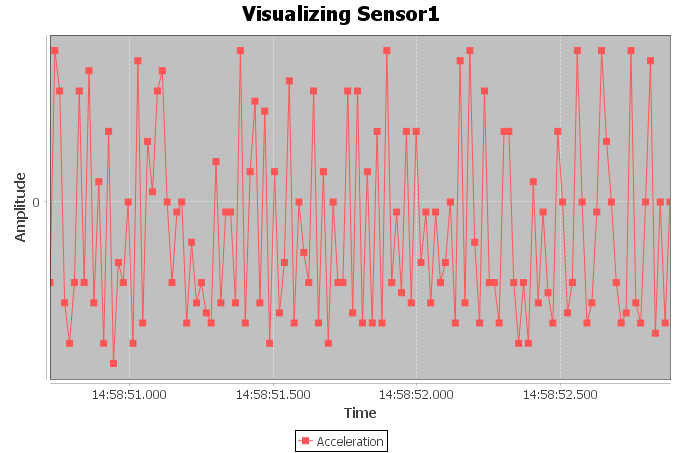
\includegraphics[scale=0.5]{ImplementasiAntarMuka/visualizing}  
	\caption[Grafik hasil implementasi visualisasi hasil sense ]{Grafik hasil implementasi visualisasi hasil sense} 
	\label{fig:implementasiV} 
\end{figure}

Gambar \ref{fig:implementasiV} menunjukkan grafik hasil {\it sensing} dari Sensor1. Grafik ini menunjukkan amplitudo dari akselerasi yang terekam
oleh Sensor1.

\subsection{Hasil Implementasi Antar Muka Spectrogram}
Berikut contoh hasil dari implementasi antar muka spectrogram hasil ekstraksi fitur dari {\it sensing} Sensor1 dengan menggunakan {\it library} dari {\it JFreeChart}. Seperti antar muka visualisasi hasil sense, pada tampilan awal (Gambar \ref{fig:implementasi1}) pengguna perlu memilih option {\it Sense}. Tampilan spectrogram akan muncul setelah sensor node mengirimkan hasil ekstrasi fitur.

\begin{figure}[H]
	\centering
	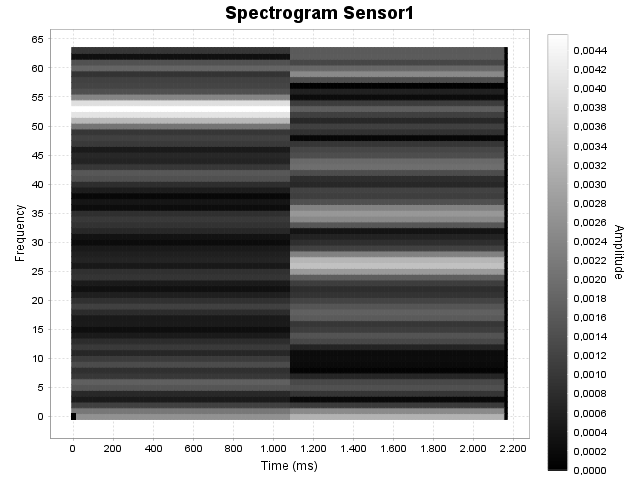
\includegraphics[scale=0.5]{ImplementasiAntarMuka/spectrogram}  
	\caption[Grafik hasil implementasi visualisasi hasil sense ]{Grafik hasil implementasi visualisasi hasil sense} 
	\label{fig:implementasiS} 
\end{figure}

Gambar \ref{fig:implementasiS} menunjukkan grafik hasil ekstraksi fitur dari hasil {\it sensing} Sensor1. Dari Grafik ini dapat terlihat frekuensi yang dominan dan frekuensi lain yang terekam dari {\it sensing} Sensor1 berdasarkan besar amplitudo dari frekuensi.

\section{Pengujian}
Pengujian dilakukan dengan menggunakan dua buah metode yaitu pengujian fungsional dan pengujian eksperimental.

\subsection{Pengujian Fungsional}
Pengujian dilakukan dengan menjalankan aplikasi di {\it Command Line Interface}. Tampilan utama setelah pengguna memasukkan jumlah sensor node seperti ada pada 
Gambar~\ref{fig:PengujianFungsional1}.
\begin{figure}[H]
	\centering
	\includegraphics[scale=1.3]{PengujianFungsional/1}  
	\caption[Tampilan awal setelah memasukkan jumlah sensor node ]{Tampilan awal setelah memasukkan jumlah sensor node} 
	\label{fig:PengujianFungsional1} 
\end{figure}

Fitur - fitur aplikasi yang terdapat pada aplikasi adalah sebagai berikut:
\begin{itemize}
\item Check Online node \\
Fitur ini berfungsi untuk menampilkan sensor node - sensor node yang sedang menyala dan menyamakan waktu pada sensor node dengan waktu yang ada
pada komputer pengguna. Untuk menjalankan fitur ini, pengguna memasukkan angka "1" dan menunggu hasil yang ditampilkan seperti pada Gambar~\ref{fig:PengujianFungsional2}.

\begin{figure}[H]
	\centering
	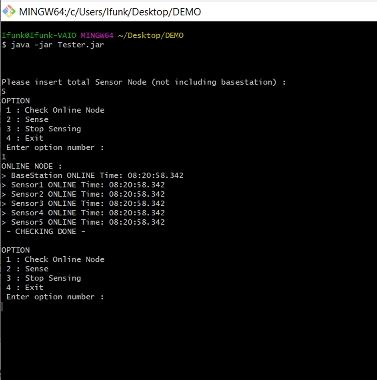
\includegraphics[scale=1.3]{PengujianFungsional/2}  
	\caption[Pengujian "Check Online node" ]{Pengujian "Check Online node"} 
	\label{fig:PengujianFungsional2} 
\end{figure}

\item Sense \\
Fitur ini berfungsi untuk memberikan perintah kepada sensor node - sensor node yang sedang menyala untuk memulai {\it sensing}. Saat pengguna memasukkan angka "2", aplikasi akan menampilkan pula grafik hasil {\it sensing} dan grafik spectrogram hasil ekstraksi fitur yang akan terus diperbaharui. Tampilan awal awal fungsi ini dijalankan seperti pada   
Gambar~\ref{fig:PengujianFungsional3} dan tampilan setelah grafik diperbaharui seperti pada Gambar~\ref{fig:PengujianFungsional4}
\begin{figure}[H]
	\centering
	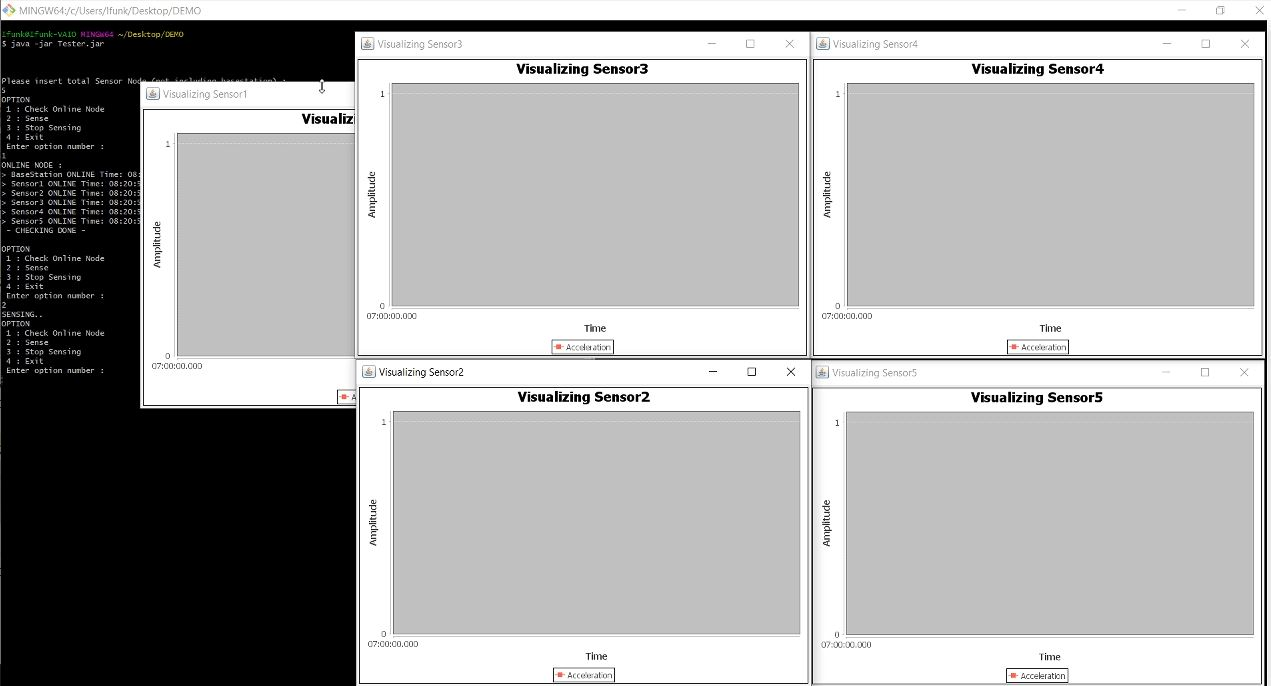
\includegraphics[scale=0.5]{PengujianFungsional/3}  
	\caption[Tampilan awal setelah menjalankan fungsi "Sense" ]{Tampilan awal setelah menjalankan fungsi "Sense"} 
	\label{fig:PengujianFungsional3} 
\end{figure}

\begin{figure}[H]
	\centering
	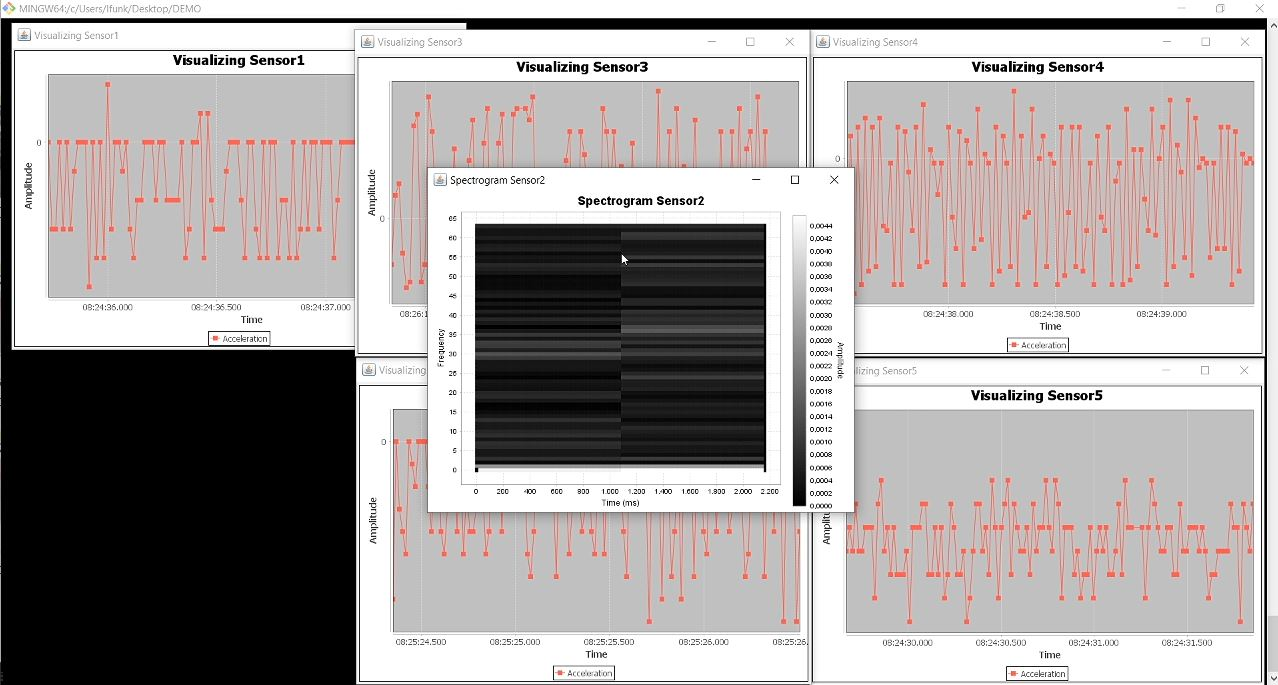
\includegraphics[scale=0.5]{PengujianFungsional/4}  
	\caption[Tampilan setelah mendapatkan hasil ekstraksi fitur dari sensor node]{Tampilan setelah mendapatkan hasil ekstraksi fitur dari sensor node} 
	\label{fig:PengujianFungsional4} 
\end{figure}

Saat fungsi Sense berjalan, aplikasi tidak akan menerima input selain masukan angka "3" untuk memberhentikan {\it sensing}. Tampilan jika pengguna memasukkan 
input lain dapat dilihat pada Gambar~\ref{fig:PengujianFungsional5}
\begin{figure}[H]
	\centering
	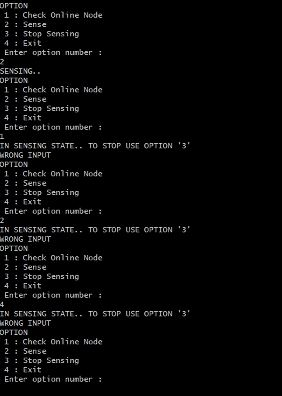
\includegraphics[scale=1.3]{PengujianFungsional/5}  
	\caption[Pengujian input selain angka "3" "Sense" ]{Pengujian input selain angka "3" saat "Sense"} 
	\label{fig:PengujianFungsional5} 
\end{figure}

\item Stop sensing \\
Fitur ini berfungsi untuk menghentikan sensor node yang sedang {\it sensing} dan menutup grafik - grafik yang ditampilkan. Pengguna harus memasukkan angka "3" saat sensor node sedang {\it sensing} untuk menjalankan fungsi ini. Tampilan setelah fungsi ini dijalankan seperti pada Gambar~\ref{fig:PengujianFungsional6}
\begin{figure}[H]
	\centering
	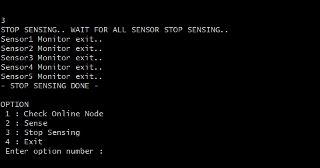
\includegraphics[scale=1.3]{PengujianFungsional/6}  
	\caption[Pengujian "Stop sensing" ]{Pengujian "Stop sensing"} 
	\label{fig:PengujianFungsional6} 
\end{figure}

\item Exit \\
Fitur ini berfungsi untuk keluar dari aplikasi. Pengguna harus memasukkan angka "4" saat sensor node tidak dalam keadaan {\it sensing} untuk menjalankan fungsi ini. Tampilan 
hasil dari fungsi in dapat dilihat pada Gambar~\ref{fig:PengujianFungsional7}
\begin{figure}[H]
	\centering
	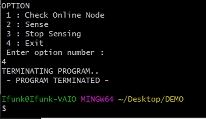
\includegraphics[scale=1.3]{PengujianFungsional/7}  
	\caption[Pengujian "Exit" ]{Pengujian "Exit"} 
	\label{fig:PengujianFungsional7} 
\end{figure}

\end{itemize}
\subsection{Pengujian Eksperimental}
Pengujian Eksperimental ini dilakukan di atap rumah penguji di jalan Pasirkaliki Bandung dan di jalan raya Pasirkaliki Bandung. Sensor node yang digunakan untuk pengujian berjumlah 6 dengan 1 sensor node sebagai {\it base station}. Arsitektur WSN yang digunakan adalah {\it flat} dengan {\it single-hop} dan {\it multi-hop}. Pengujian dilakukan untuk melihat kemampuan sensor node mengekstraksi fitur di atap rumah dan di jalan raya dengan topologi {\it star} dan topologi {\it tree}. Pengujian ini mengukur sumbu $x$ dari akselerometer untuk {\it sample} sebesar 128 dalam 2 detik, {\it window} sebesar 64, {\it overlap} sebesar 0\%, dan {\it sampling rate} sebesar $64 Sample/second$. 
Pengujian ini menggunakan {\it Window function} {\it Rectangle}, {\it Hanning}, dan {\it Hamming}. Besar {\it sample} dan {\it window function} tersebut dipilih untuk melihat kemampuan aplikasi ini dalam melakukan ekstraksi fitur di sensor node  dengan besar {\it sample} dan {\it window} tersebut. Dengan {\it sampling rate} setengah dari besar {\it sample} maka setiap frekuensi getaran yang didapat adalah setengah dari frekuensi getaran yang didapat. 

Topologi yang digunakan untuk pengujian ini adalah topologi {\it star} (Gambar~\ref{fig:PengujianEksperimentaltopologistar}) dan {\it tree} (Gambar~\ref{fig:PengujianEksperimentaltopologitree}). Topologi {\it star} dan {\it tree} dipilih karena kedua topologi tersebut sudah mencakup 2 jalur komunikasi WSN ({\it single hop} dan {\it multi hop}).

\begin{figure}[H]
	\centering
	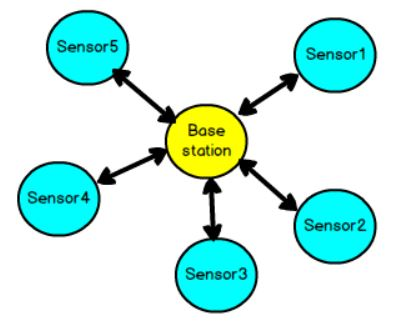
\includegraphics[scale=0.8]{PengujianEksperimental/topologistar}  
	\caption[Topologi star yang digunakan]{Topologi star yang digunakan} 
	\label{fig:PengujianEksperimentaltopologistar} 
\end{figure}

\begin{figure}[H]
	\centering
	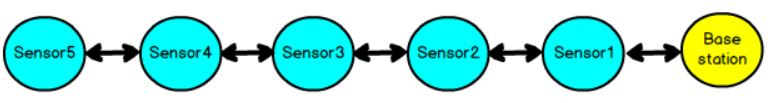
\includegraphics[scale=0.8]{PengujianEksperimental/topologitree}  
	\caption[Topologi tree yang digunakan]{Topologi tree yang digunakan} 
	\label{fig:PengujianEksperimentaltopologitree} 
\end{figure}

Skenario - skenario dalam pengujian ini berfokus dalam menguji setiap topologi dan {\it window function} yang digunakan. Setiap skenario bertujuan melihat kemampuan ekstraksi fitur setiap sensor node. Langkah pengujian pada setiap skenario dalam pengujian ini adalah sebagai berikut:
\begin{enumerate}
	\item Sensor node diatur dengan topologi dan {\it window function} tertentu.
	\item Sensor node diletakkan ditempat yang berjauhan dan sama pada setiap skenario.
	\item Mengecek status {\it online} setiap sensor node lewat komputer.
	\item Memberi perintah {\it sense} ke setiap sensor node lewat komputer.
	\item Hasil tampilan dari hasil ekstraksi fitur di simpan 
\end{enumerate}
Hasil dari pengujian ini berupa grafik amplitudo akselerasi dari hasil {\it sensing} dan grafik spectrogram hasil ekstraksi fitur dari setiap sensor node.  

\subsubsection{Pengujian di Atap Rumah}
Pada pengujian ini sensor diletakkan seperti pada Gambar~\ref{fig:PengujianEksperimentaldenah}. Setiap sensor node diberi jarak satu sama lain untuk menunjukkan komunikasi setiap sensor node secara nirkabel dan untuk melihat hasil ekstraksi di lokasi - lokasi yang berbeda. 

\begin{figure}[H]
	\centering
	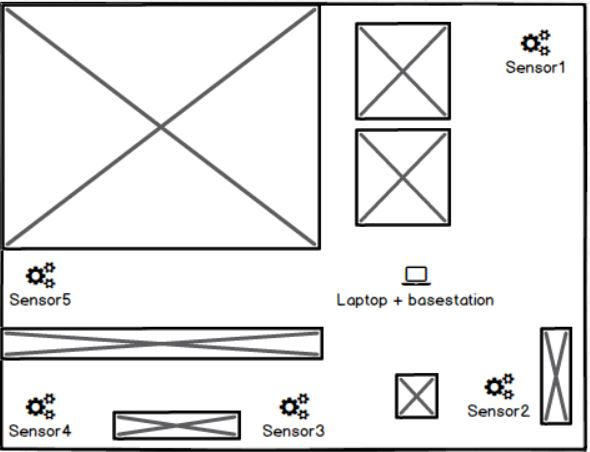
\includegraphics[scale=1]{PengujianEksperimental/denah}  
	\caption[Denah peletakkan sensor node]{Denah peletakkan sensor node} 
	\label{fig:PengujianEksperimentaldenah} 
\end{figure}

Pengujian dilakukan saat pagi ke siang hari dengan cuaca berawan. Hasil grafik dari pengujian dapat di lihat pada lampiran \ref{lamp:B}.

\begin{itemize}
\item Topologi Star\\
\begin{table}[H]
    \centering
    \caption{Tabel hasil getaran yang tertangkap di Atap dengan Topologi Star}
    \begin{tabular}{|p{3cm}|p{3cm}|p{3cm}|p{3cm}|p{3cm}|}
    \hline Id Sensor & frekuensi dominan saat 0ms ($Hz$)& frekuensi dominan saat 1000ms ($Hz$)& {\it window function}\\
    \hline Sensor1 & 0& 0.5 & {\it Rectangle} \\
    \hline Sensor2 & 0& 0.5 & {\it Rectangle} \\
    \hline Sensor3 & 9 & 9 & {\it Rectangle} \\
    \hline Sensor4 & 0 & 0.5 & {\it Rectangle} \\
    \hline Sensor5 & 0 & 0.5 & {\it Rectangle} \\
    \hline Sensor1 & 24.5& 27.5 & {\it Hanning} \\
    \hline Sensor2 & 17.5 &17.5 & {\it Hanning} \\
    \hline Sensor3 &2 & 0& {\it Hanning} \\
    \hline Sensor4 & 0& 0.5& {\it Hanning} \\
    \hline Sensor5 &0 & 0& {\it Hanning} \\
    \hline Sensor1 & 15& 11& {\it Hamming} \\
    \hline Sensor2 &0 & 0.5 & {\it Hamming} \\
    \hline Sensor3 &0 &0 & {\it Hamming} \\
    \hline Sensor4 &0 &0 & {\it Hamming} \\
    \hline Sensor5 &0 &0 & {\it Hamming} \\
    \hline
    \end{tabular}
    \label{tab:starAtapResult}
\end{table}

\item Topologi Tree\\
Berikut tabel dari hasil getaran yang terekam oleh sensor node di atap rumah dengan topologi {\it tree}.

\begin{table}[H]
    \centering
    \caption{Tabel hasil getaran yang tertangkap di Atap dengan Topologi Tree}
    \begin{tabular}{|p{3cm}|p{3cm}|p{3cm}|p{3cm}|p{3cm}|}
    \hline Id Sensor & frekuensi dominan saat 0ms ($Hz$)& frekuensi dominan saat 1000ms ($Hz$)& {\it window function}\\
    \hline Sensor1 & 0 & 0 & {\it Rectangle} \\
    \hline Sensor2 & 0 & 0 & {\it Rectangle} \\
    \hline Sensor3 & 1 & 0 & {\it Rectangle} \\
    \hline Sensor4 & 0 & 0 & {\it Rectangle} \\
    \hline Sensor5 & 0 & 0 & {\it Rectangle} \\
    \hline Sensor1 & 0 & 0 & {\it Hanning} \\
    \hline Sensor2 & 0 & 0 & {\it Hanning} \\
    \hline Sensor3 & 31.5 & 31.5 & {\it Hanning} \\
    \hline Sensor4 & 0 & 0 & {\it Hanning} \\
    \hline Sensor5 & 0 & 0 & {\it Hanning} \\
    \hline Sensor1 & 0 & 0 & {\it Hamming} \\
    \hline Sensor2 & 0 & 0 & {\it Hamming} \\
    \hline Sensor3 & 22 & 10 & {\it Hamming} \\
    \hline Sensor4 & 0 & 0 & {\it Hamming} \\
    \hline Sensor5 & 0 & 0 & {\it Hamming} \\
    \hline
    \end{tabular}
    \label{tab:treeAtapResult}
\end{table}

Dari tabel \ref{tab:starAtapResult} dan \ref{tab:treeAtapResult} terlihat bahwa sensor node berhasil merekam getaran dan frekuensi dari atap rumah dengan topologi tree. Hasil frekuensi dari sensor yang berbeda - beda disebabkan karena perbedaan tempat dan waktu saat melakukan {\it sensing} sehingga getaran yang ditangkap berbeda - beda. Getaran terbesar yang ditangkap oleh sensor di Atap adalah sebesar $31.5Hz$ dan getaran terendah adalah $0Hz$.
\end{itemize}

\subsubsection{Pengujian di Jalan Raya}
Pada pengujian ini sensor node diletakkan di pinggir jalan untuk merekam getaran - getaran saat ada kendaraan yang melewatinya. Hasil dari pengujian dapat di lihat pada lampiran \ref{lamp:C}.

\begin{itemize}
\item Topologi Star\\
Pengujian dilakukan dengan kondisi jalan raya cukup sepi. Berikut tabel dari hasil getaran yang terekam oleh sensor node di jalan raya dengan topologi {\it star}.

\begin{table}[H]
    \centering
    \caption{Tabel hasil getaran yang tertangkap di Jalan Raya dengan Topologi Star}
    \begin{tabular}{|p{3cm}|p{3cm}|p{3cm}|p{3cm}|p{3cm}|}
    \hline Id Sensor & frekuensi dominan saat 0ms ($Hz$)& frekuensi dominan saat 1000ms ($Hz$)& {\it window function}\\
    \hline Sensor1 & 0 & 0 & {\it Rectangle} \\
    \hline Sensor2 & 0 & 9 & {\it Rectangle} \\
    \hline Sensor3 & 0 & 0 & {\it Rectangle} \\
    \hline Sensor4 & 0 & 26 & {\it Rectangle} \\
    \hline Sensor5 & 0 & 0 & {\it Rectangle} \\
    \hline Sensor1 & 0 & 18 & {\it Hanning} \\
    \hline Sensor2 & 0 & 0 & {\it Hanning} \\
    \hline Sensor3 & 15 & 11.5 & {\it Hanning} \\
    \hline Sensor4 & 0 & 0 & {\it Hanning} \\
    \hline Sensor5 & 0 & 0 & {\it Hanning} \\
    \hline Sensor1 & 26.5 & 13 & {\it Hamming} \\
    \hline Sensor2 & 0 & 0 & {\it Hamming} \\
    \hline Sensor3 & 22 & 10 & {\it Hamming} \\
    \hline Sensor4 & 0 & 0 & {\it Hamming} \\
    \hline Sensor5 & 0 & 0 & {\it Hamming} \\
    \hline
    \end{tabular}
    \label{tab:starRoadResult}
\end{table}


\item Topologi Tree\\
\begin{table}[H]
    \centering
    \caption{Tabel hasil getaran yang tertangkap di Jalan Raya dengan Topologi Tree}
    \begin{tabular}{|p{3cm}|p{3cm}|p{3cm}|p{3cm}|p{3cm}|}
    \hline Id Sensor & frekuensi dominan saat 0ms ($Hz$)& frekuensi dominan saat 1000ms ($Hz$)& {\it window function}\\
    \hline Sensor1 & 0 & 0 & {\it Rectangle} \\
    \hline Sensor2 & 30.5 & 31.5 & {\it Rectangle} \\
    \hline Sensor3 & 0 & 0 & {\it Rectangle} \\
    \hline Sensor4 & 2 & 7.5 & {\it Rectangle} \\
    \hline Sensor5 & 0 & 0 & {\it Rectangle} \\
    \hline Sensor1 & 0 & 0 & {\it Hanning} \\
    \hline Sensor2 & 0 & 0 & {\it Hanning} \\
    \hline Sensor3 & 0 & 0 & {\it Hanning} \\
    \hline Sensor4 & 19 & 10 & {\it Hanning} \\
    \hline Sensor5 & 0 & 0 & {\it Hanning} \\
    \hline Sensor1 & 0 & 0 & {\it Hamming} \\
    \hline Sensor2 & 10.5 & 26.5 & {\it Hamming} \\
    \hline Sensor3 & 0 & 11 & {\it Hamming} \\
    \hline Sensor4 & 7 & 0 & {\it Hamming} \\
    \hline Sensor5 & 0 & 0 & {\it Hamming} \\
    \hline
    \end{tabular}
    \label{tab:treeRoadResult}
\end{table}
\end{itemize}

Dari tabel \ref{tab:starRoadResult} dan \ref{tab:treeRoadResult} terlihat bahwa sensor node berhasil merekam getaran dan frekuensi dari jalan raya dengan topologi star dan tree. Hasil frekuensi dari sensor yang berbeda - beda disebabkan karena perbedaan tempat dan waktu saat melakukan {\it sensing} sehingga getaran yang ditangkap berbeda - beda. Getaran terbesar yang terekam di jalan raya adalah $31.5Hz$ dan getaran terendah adalah $0Hz$.  

\subsubsection{Kesimpulan dari Pengujian}
Dari hasil eksperimen, aplikasi berhasil melakukan ekstraksi fitur di atap dan jalan raya dengan topologi {\it star} dan {\it tree}. Getaran terendah yang ditangkap sensor di atap dan jalan raya adalah getaran dengan frekuensi $0Hz$ dan getaran terbesarnya dengan frekuensi $31.5Hz$.
Dari pengujian ini terlihat bahwa hasil ekstraksi fitur tidak terpengaruh oleh topologi dari WSN yang dipakai namun dari tempat dan letak sensor node melakukan {\it sensing}.

\subsection{Masalah dalam Pengujian}
Berikut masalah - masalah yang dihadapi saat penguji melakukan pengujian:
\begin{enumerate}
	\item Sensor node yang digunakan untuk pengujian terbatas, sehingga sensor node harus dipakai secara bergantian dengan mahasiswa lain yang 
		mengambil topik skripsi yang berkaitan dengan sensor node. 
	\item {\it Memory} minim pada sensor node yang menghambat proses ekstraksi fitur yang membutuhkan memory yang besar untuk menyimpan {\it sample} dan hasil dari {\it ekstraksi fitur}
	\item Saat pengujian sensor node dapat mati secara tiba - tiba, karena sumber {\it power} dari sensor node (baterai) dapat habis saat sensor node melakukan {\it sensing}
	\item Cuaca hujan yang menghambat pengujian, karena pengujian dilakukan di ruangan terbuka. 
	\item Pengujian dilakukan saat adanya pandemi virus {\it Covid19}, sehingga adanya keterbatasan untuk keluar rumah dan penggunaan sensor node
		secara bersama dengan mahasiswa lain yang memilih topik skripsi yang berkaitan demi mematuhi peraturan PSBB (Pembatasan Sosial Berskala Besar) dari pemerintah.  
\end{enumerate}
	


